\documentclass[aspectratio=169, table]{beamer}

%\usepackage[beamertheme=./praditatheme]{Pradita}
\usepackage[utf8]{inputenc}
\usepackage{xcolor} % for color
\usepackage{colortbl} % for table color
\usepackage{listings}

% Define Java language style for listings
\lstdefinestyle{JavaStyle}{
language=Java,
basicstyle=\ttfamily\scriptsize,
keywordstyle=\color{blue},
commentstyle=\color{gray},
stringstyle=\color{red},
breaklines=true,
showstringspaces=false,
tabsize=2,
captionpos=b,
numbers=left,
numberstyle=\tiny\color{gray},
frame=lines,
backgroundcolor=\color{lightgray!10},
comment=[l]{//},
morecomment=[s]{/*}{*/},
commentstyle=\color{gray}\ttfamily,
string=[s]{'}{'},
morestring=[s]{"}{"},
%	stringstyle=\color{teal}\ttfamily,
%	showstringspaces=false
}

\usetheme{Pradita}
%
\subtitle{IF220303 - Object-oriented Programming}

\title{\Huge{Behavioral Patterns 1}\\\vspace{30pt}}
\date[Serial]{\scriptsize {PRU/SPMI/FR-BM-18/0222}}
\author[Pradita]{\small {\textbf{Alfa Yohannis}}}

\begin{document}

\frame{\titlepage}

\begin{frame}[fragile]
\frametitle{Contents}
\vspace{20pt}
\begin{columns}[t]
\column{0.5\textwidth}
\tableofcontents[sections={1-3}]

\column{0.5\textwidth}
\tableofcontents[sections={4-5}]
\end{columns}
\end{frame}


\section{Pola Desain Perilaku}

\begin{frame}{Pola Desain Perilaku}
	\vspace{10pt}
	Pola desain perilaku (\textit{behavioral design patterns}) adalah pendekatan dalam OOP yang menekankan interaksi antar objek dan distribusi tanggung jawab secara dinamis.
	
	\vspace{10pt}
	Bab ini membahas empat pola perilaku utama:
	\begin{itemize}
		\item \textbf{Interpreter:} Mendefinisikan dan mengevaluasi struktur ekspresi atau bahasa.
		\item \textbf{Observer:} Menyebarkan notifikasi perubahan status secara otomatis.
		\item \textbf{Strategy:} Memungkinkan pemilihan algoritma yang dapat diganti saat runtime.
		\item \textbf{Command:} Membungkus aksi sebagai objek mandiri.
	\end{itemize}
	
	\vspace{5pt}
	Pola-pola ini membantu menciptakan sistem yang modular, fleksibel, dan mudah dipelihara.
\end{frame}


\section{Pola Interpreter}

\begin{frame}{\hfill}
	\centering
	\textbf{\Huge{Pola Interpreter}}
\end{frame}

\begin{frame}{Interpreter: Tujuan dan Konteks Penggunaan}
	\vspace{15pt}
	Pola \textit{Interpreter} mendefinisikan grammar dan cara interpretasi kalimat. Cocok untuk ekspresi berulang seperti matematika atau logika sederhana, tapi kurang efektif untuk grammar kompleks karena struktur kelas yang dalam.
	
	\vspace{5pt}
	\begin{columns}[T]
		\column{0.5\textwidth}
		\textbf{Tujuan:}
		\begin{itemize}
			\item Definisikan grammar dan ekspresi.
			\item Sediakan antarmuka interpretasi.
			\item Pisahkan logika evaluasi dari data.
		\end{itemize}
		
		\textbf{Struktur:}
		\begin{itemize}
			\item \textbf{AbstractExpression}
			\item \textbf{TerminalExpression}
			\item \textbf{NonTerminalExpression}
			\item \textbf{Context}
		\end{itemize}
		
		\column{0.5\textwidth}
		\textbf{Kapan Digunakan:}
		\begin{itemize}
			\item Grammar stabil dan simpel.
			\item Butuh interpretasi langsung.
			\item Evaluasi ekspresi pohon.
		\end{itemize}
		
		\textbf{Contoh:}
		\begin{itemize}
			\item Kalkulator ekspresi.
			\item Filter logika sederhana.
			\item Mini query pada data.
			\item Bahasa skrip/DSL kecil.
		\end{itemize}
	\end{columns}
	
\end{frame}


\begin{frame}{Interpreter: Contoh Kasus Penggunaan}
	\vspace{20pt}
Pola \textit{Interpreter} cocok untuk evaluasi ekspresi sederhana: kalkulator, query, DSL.
	
%	\vspace{5pt}
	\begin{itemize}
		\item \textbf{Kalkulator Ekspresi Aritmatika:} Ekspresi seperti \texttt{(5 + 3) - 2} diproses sebagai pohon dan diinterpretasi secara rekursif.
		\item \textbf{Query Filter dan Pencarian Data:} Ekspresi seperti \texttt{name = 'Alice' AND age > 25} diuraikan ke dalam ekspresi terminal dan non-terminal.
		\item \textbf{Bahasa Domain Khusus (DSL):} DSL seperti \texttt{IF order.total > 500 THEN apply\_discount} diinterpretasikan langsung terhadap struktur data.
		\item \textbf{Sistem Validasi dan Aturan:} Digunakan dalam rule engine untuk mengevaluasi kebijakan berbasis data klien.
		\item \textbf{AI Game Logic:} Evaluasi kondisi seperti \texttt{EnemyInRange AND HasAmmo} dalam sistem pengambilan keputusan karakter.
		\item \textbf{Parsing Format Ringan:} Ekspresi postfix, prefix, atau konfigurasi seperti JSONPath/XPath diproses sebagai pohon ekspresi.
	\end{itemize}

\end{frame}


\begin{frame}{Interpreter: Kelebihan dan Kekurangan}
	\vspace{10pt}
	\begin{columns}[T]
		\column{0.5\textwidth}
		\textbf{Kelebihan:}
		\begin{itemize}
			\item Mudah dikembangkan dan diperluas.
			\item Cocok untuk DSL kecil dan stabil.
			\item Struktur ekspresi modular dan hierarkis.
			\item Memisahkan logika evaluasi dari data.
			\item Implementasi eksplisit, mudah ditelusuri.
		\end{itemize}
		
		\column{0.5\textwidth}
		\textbf{Kekurangan:}
		\begin{itemize}
			\item Kurang efisien untuk grammar besar.
			\item Proliferasi kelas kecil sulit dikelola.
			\item Tidak fleksibel untuk grammar dinamis.
			\item Debugging sulit pada ekspresi dalam.
			\item Sulit dioptimasi secara menyeluruh.
		\end{itemize}
	\end{columns}
	
	\vspace{6pt}
	\small Cocok untuk evaluator kecil dan DSL statis. Gunakan parser atau AST untuk grammar kompleks dan sistem performa tinggi.
\end{frame}

\begin{frame}{Struktur Pola Interpreter}
	\vspace{10pt}
	\centering
	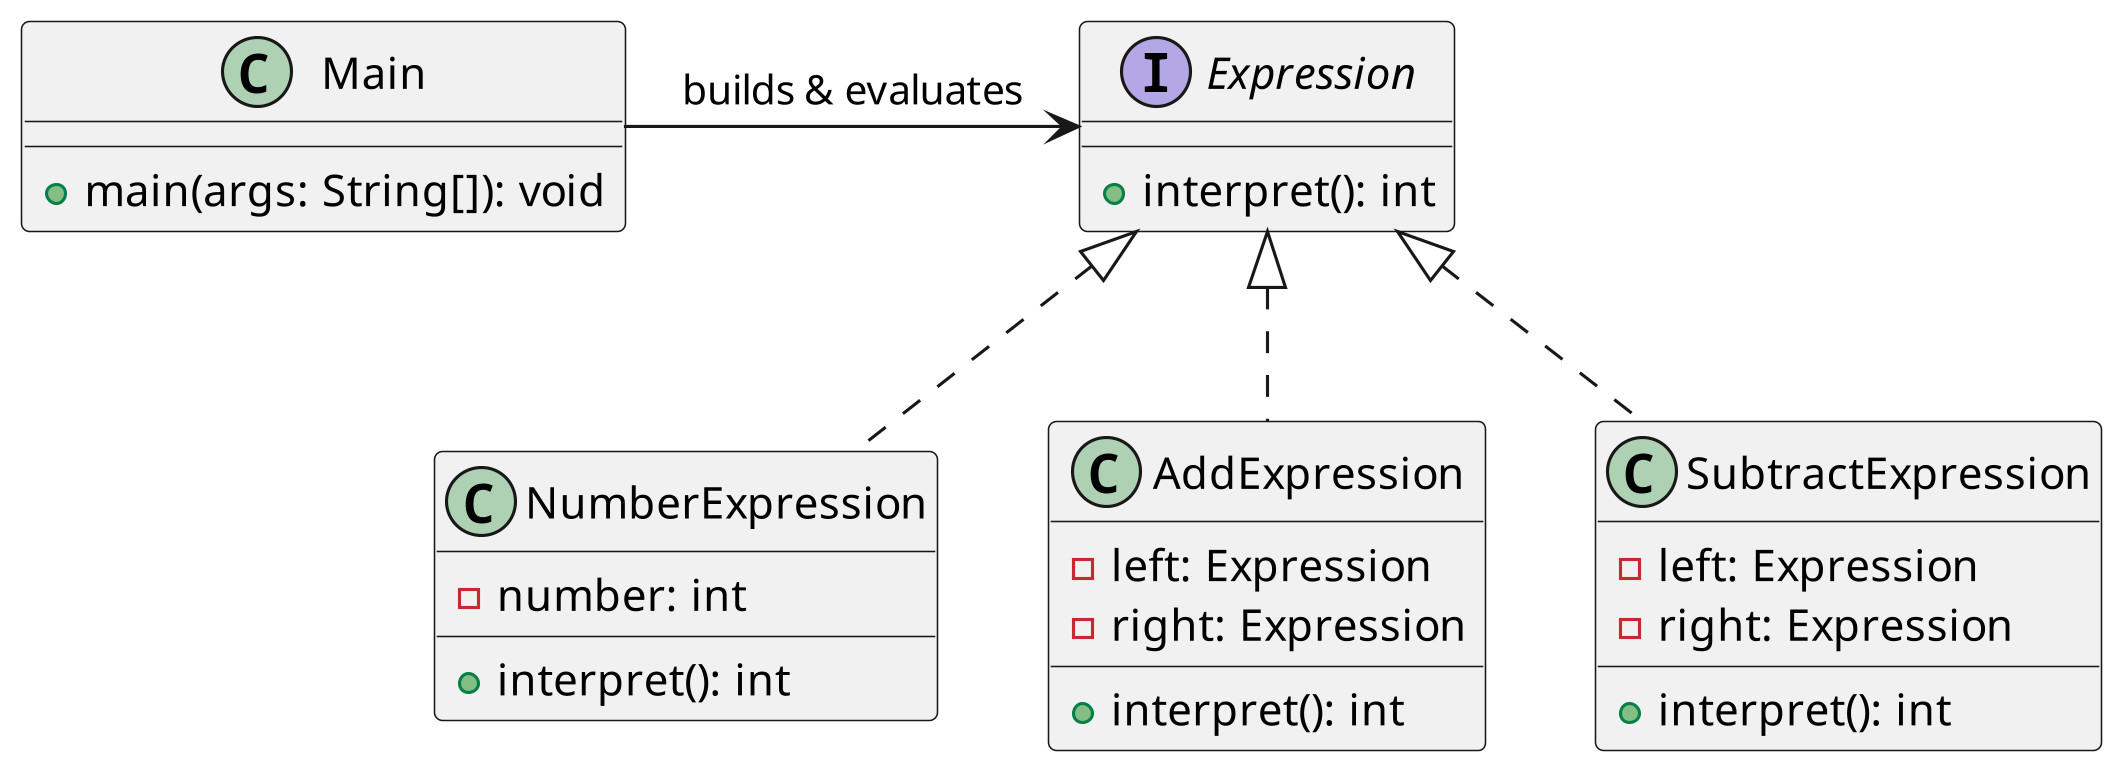
\includegraphics[width=\textwidth]{../../figures/out/interpreter.png}
	
	\vspace{10pt}
	\small
	Struktur menunjukkan bagaimana \texttt{Client} membangun dan mengevaluasi pohon ekspresi menggunakan \texttt{interpret()} secara rekursif. \texttt{Context} menyediakan informasi global saat interpretasi berlangsung.
\end{frame}



\begin{frame}[fragile]{Antarmuka Ekspresi}
	\begin{lstlisting}[style=JavaStyle]
		public interface Expression {
			int interpret();
		}
	\end{lstlisting}
	\small
	\texttt{Expression} adalah antarmuka umum untuk semua jenis ekspresi yang dapat dievaluasi. Setiap implementasi akan mendefinisikan metode \texttt{interpret()}.
\end{frame}

\begin{frame}[fragile]{Ekspresi Konstanta (Terminal)}
	\begin{lstlisting}[style=JavaStyle]
		public class NumberExpression implements Expression {
			private int number;
			
			public NumberExpression(int number) {
				this.number = number;
			}
			
			@Override
			public int interpret() {
				return number;
			}
		}
	\end{lstlisting}
	\small
	\texttt{NumberExpression} mewakili nilai konstan sebagai simbol terminal dalam grammar, dan langsung mengembalikan nilainya saat dievaluasi.
\end{frame}

\begin{frame}[fragile]{Ekspresi Penjumlahan (Non-Terminal)}
	\begin{lstlisting}[style=JavaStyle]
		public class AddExpression implements Expression {
			private Expression left;
			private Expression right;
			
			public AddExpression(Expression left, Expression right) {
				this.left = left;
				this.right = right;
			}
			
			@Override
			public int interpret() {
				return left.interpret() + right.interpret();
			}
		}
	\end{lstlisting}
	\small
	\texttt{AddExpression} adalah ekspresi komposit yang menjumlahkan dua ekspresi lainnya secara rekursif.
\end{frame}

\begin{frame}[fragile]{Ekspresi Pengurangan (Non-Terminal)}
	\begin{lstlisting}[style=JavaStyle]
		public class SubtractExpression implements Expression {
			private Expression left;
			private Expression right;
			
			public SubtractExpression(Expression left, Expression right) {
				this.left = left;
				this.right = right;
			}
			
			@Override
			public int interpret() {
				return left.interpret() - right.interpret();
			}
		}
	\end{lstlisting}
	\small
	\texttt{SubtractExpression} mengimplementasikan pengurangan dua ekspresi sebagai bagian dari struktur ekspresi pohon.
\end{frame}

\begin{frame}[fragile]{Client: Evaluasi Ekspresi}
	\begin{lstlisting}[style=JavaStyle]
		public class Main {
			public static void main(String[] args) {
				Expression expr = new AddExpression(
				new NumberExpression(10),
				new SubtractExpression(
				new NumberExpression(5),
				new NumberExpression(2)
				)
				);
				
				System.out.println("Result: " + expr.interpret()); // Output: 13
			}
		}
	\end{lstlisting}
	\small
	Ekspresi komposit \texttt{(10 + (5 - 2))} dibentuk sebagai pohon dan dievaluasi secara rekursif untuk menghasilkan hasil akhir.
\end{frame}

\section{Pola Observer}

\begin{frame}{\hfill}
	\centering
	\textbf{\Huge{Pola Observer}}
\end{frame}

\begin{frame}{Observer: Tujuan dan Konteks Penggunaan}
	\vspace{15pt}
	Pola \textit{Observer} mendefinisikan relasi satu-ke-banyak, di mana perubahan pada satu objek (\texttt{Subject}) otomatis menotifikasi semua objek terkait (\texttt{Observer}).
	
	\vspace{5pt}
	\begin{columns}[T]
		\column{0.5\textwidth}
		\textbf{Kapan Digunakan:}
		\begin{itemize}
			\item Data sering berubah dan perlu disebar ke banyak bagian.
			\item Sistem berbasis event atau reaktif.
			\item Perlu memisahkan data dan tampilan (MVC).
		\end{itemize}
		\textbf{Manfaat:}
		\begin{itemize}
			\item Mendukung \textit{loose coupling}.
			\item Menjaga konsistensi antar objek.
			\item Modular dan mudah dikembangkan.
		\end{itemize}
		
		
		
		\column{0.5\textwidth}
		\textbf{Komponen Utama:}
		\begin{enumerate}
			\item \textbf{Subject}: Menyimpan state dan daftar observer.
			\item \textbf{Observer}: Merespons perubahan state.
			\item \textbf{ConcreteSubject \& ConcreteObserver}.
		\end{enumerate}
		\textbf{Contoh Aplikasi:}
		\begin{itemize}
			\item GUI (Swing, JavaFX)
			\item Event handler
			\item Publish-subscribe
		\end{itemize}
	\end{columns}
\end{frame}


\begin{frame}{Observer: Contoh Kasus Penggunaan}
	\vspace{10pt}
	Pola \textit{Observer} umum digunakan untuk notifikasi otomatis saat status objek berubah. Cocok untuk sistem dinamis dan terpisah secara logika.
	
	\vspace{6pt}
	\begin{itemize}
		\item \textbf{UI (User Interface):} View langsung memperbarui diri saat model berubah (pola MVC).
		
		\item \textbf{Event Handling:} Tombol memberi tahu listener, umum di Swing/AWT.
		
		\item \textbf{Sinkronisasi Komponen:} Perubahan satu elemen memperbarui elemen lain, misalnya grafik.
		
		\item \textbf{Notifikasi:} Media sosial atau berita memberi tahu saat topik diperbarui.
		
		\item \textbf{Monitoring:} Modul log atau kirim alert saat status layanan berubah.
		
		\item \textbf{Data Feed:} Harga saham dikirim real-time ke observer yang terdaftar.
	\end{itemize}
\end{frame}

\begin{frame}{Observer: Kelebihan dan Kekurangan}
	\vspace{10pt}
	\begin{columns}[T]
		\column{0.5\textwidth}
		\textbf{Kelebihan:}
		\begin{itemize}
			\item \textbf{Dekopling Subject–Observer:} Meningkatkan modularitas dan fleksibilitas.
			\item \textbf{Notifikasi otomatis:} Data dan tampilan selalu sinkron.
			\item \textbf{Mudah diperluas:} Tambah observer tanpa ubah subject.
			\item \textbf{Reaktif dan event-driven:} Cocok untuk sistem real-time.
			\item \textbf{Didukung luas:} Ada di Java, C\#, dan framework lainnya.
		\end{itemize}
		
		\column{0.5\textwidth}
		\textbf{Kekurangan:}
		\begin{itemize}
			\item \textbf{Sulit ditelusuri dan diuji:} Alur update tersebar.
			\item \textbf{Masalah performa:} Terjadi jika observer banyak atau berat.
			\item \textbf{Keterkaitan implisit:} Potensi efek tak terduga.
			\item \textbf{Memory leaks:} Jika observer tidak dihapus eksplisit.
			\item \textbf{Urutan update tidak terjamin:} Dapat menyebabkan inkonsistensi.
		\end{itemize}
	\end{columns}
	
	\vspace{5pt}
	Efektif untuk sistem modular dan reaktif, tapi perlu pengelolaan agar tetap skalabel.
\end{frame}

\begin{frame}{Struktur Pola Observer}
	\vspace{20pt}
	\centering
	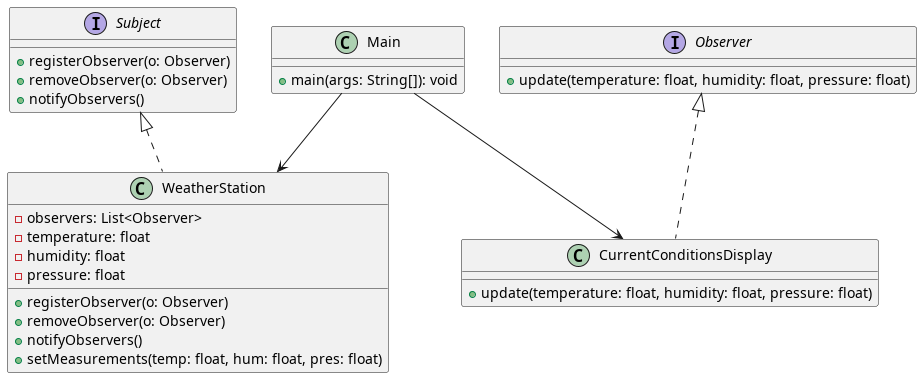
\includegraphics[width=.9\textwidth]{../../figures/out/observer.png}
	
	Diagram menunjukkan hubungan antara \texttt{Subject}, \texttt{Observer}, dan implementasi konkretnya.
\end{frame}

\begin{frame}[fragile]{Observer: Antarmuka Subject dan Observer}
	\begin{lstlisting}[style=JavaStyle]
		public interface Observer {
			void update(float temperature, float humidity, float pressure);
		}
		
		public interface Subject {
			void registerObserver(Observer o);
			void removeObserver(Observer o);
			void notifyObservers();
		}
	\end{lstlisting}
	\small Dua antarmuka mendefinisikan kontrak untuk hubungan antara objek pengamat dan objek yang diamati.
\end{frame}

\begin{frame}[fragile]{Observer: WeatherStation sebagai Subject}
	\vspace{10pt}
\begin{columns}[T]
\column{0.5\textwidth}
\begin{lstlisting}[style=JavaStyle]
import java.util.*;

public class WeatherStation 
implements Subject {
	private List<Observer> observers 
	= new ArrayList<>();
	private float temperature, 
	humidity, pressure;
	public void registerObserver(Observer o) {
		observers.add(o);
	}
	public void removeObserver(Observer o) {
		observers.remove(o);
	}
\end{lstlisting}

\column{0.5\textwidth}
\begin{lstlisting}[style=JavaStyle]
	public void notifyObservers() {
		for (Observer o : observers) {
			o.update(temperature, 
			humidity, 
			pressure);
		}
	}
	public void setMeasurements(
	float temp, float hum, float pres) {
		this.temperature = temp;
		this.humidity = hum;
		this.pressure = pres;
		notifyObservers();
	}
}
\end{lstlisting}
\end{columns}

\vspace{4pt}
\small Kelas \texttt{WeatherStation} bertindak sebagai pusat data yang memberi tahu semua observer saat data cuaca berubah.
\end{frame}


\begin{frame}[fragile]{Observer: Implementasi CurrentConditionsDisplay}
	\begin{lstlisting}[style=JavaStyle]
		public class CurrentConditionsDisplay implements Observer {
			@Override
			public void update(float temperature, float humidity, float pressure) {
				System.out.println("Current Conditions: " + temperature + 
				" C, " + humidity + "% humidity, " + pressure + " hPa");
			}
		}
	\end{lstlisting}
	\small Kelas \texttt{CurrentConditionsDisplay} mencetak data terbaru saat menerima notifikasi dari \texttt{WeatherStation}.
\end{frame}

\begin{frame}[fragile]{Observer: Client}
	\begin{lstlisting}[style=JavaStyle]
		public class Main {
			public static void main(String[] args) {
				WeatherStation station = new WeatherStation();
				Observer display = new CurrentConditionsDisplay();
				
				station.registerObserver(display);
				station.setMeasurements(26.5f, 65f, 1012f);
			}
		}
	\end{lstlisting}
	\small Objek \texttt{display} mendaftar ke \texttt{station} dan otomatis menerima pembaruan ketika data berubah.
\end{frame}


\section{Pola Strategy}

\begin{frame}{\hfill}
	\centering
	\textbf{\Huge{Pola Strategy}}
\end{frame}

\begin{frame}{Strategy: Tujuan dan Konteks Penggunaan}
	\vspace{20pt}
	Pola \textit{Strategy} memisahkan algoritma dari objek. Algoritma dibungkus dalam kelas terpisah dan dapat diganti dinamis tanpa ubah kode utama. 
	\vspace{1pt}
	\begin{columns}[T]
		\column{0.5\textwidth}
		\textbf{Tujuan:}
		\begin{itemize}
			\item Hindari struktur \texttt{if-else} kompleks.
			\item Pilih algoritma saat runtime.
			\item Pisahkan tanggung jawab logika dan eksekusi.
		\end{itemize}
		
		\textbf{Struktur:}
		\begin{itemize}
			\item \textbf{Strategy:} Antarmuka umum.
			\item \textbf{ConcreteStrategy:} Implementasi algoritma.
			\item \textbf{Context:} Mengatur strategi.
		\end{itemize}
		
		\column{0.5\textwidth}
		\textbf{Kapan Digunakan:}
		\begin{itemize}
			\item Banyak algoritma serupa perlu dikelola modular.
			\item Ingin ekstensi tanpa ubah kode klien.
			\item Perilaku algoritmik sering berubah.
		\end{itemize}
		
		\textbf{Contoh Aplikasi:}
		\begin{itemize}
			\item Metode pembayaran (e-wallet, kartu).
			\item Kompresi file (zip, rar, 7z).
			\item Biaya pengiriman (berat, jarak, layanan).
		\end{itemize}
	\end{columns}

\end{frame}

\begin{frame}{Strategy: Contoh Kasus Penggunaan}
	\vspace{10pt}
	Pola \textit{Strategy} digunakan saat ada beberapa cara menyelesaikan tugas dan pemilihannya bersifat dinamis. Dengan memisahkan algoritma dalam kelas terpisah, sistem menjadi modular, fleksibel, dan mudah diuji. Cocok untuk sistem yang sering berubah karena mudah diperluas tanpa modifikasi.
	
	\vspace{6pt}
	\begin{itemize}
		\item \textbf{Pembayaran Online:} Kartu kredit, e-wallet, dan transfer bank dikemas sebagai strategi berbeda.
		\item \textbf{Kompresi File:} ZIP, RAR, dan 7z sebagai strategi kompresi yang dipilih dinamis.
		\item \textbf{Tarif Pengiriman:} Hitung berdasarkan berat, jarak, atau jenis layanan.
		\item \textbf{Sorting Data:} Urutkan berdasarkan nama, tanggal, atau prioritas.
		\item \textbf{Game AI:} Strategi menyerang, bertahan, atau eksplorasi sesuai kondisi.
		\item \textbf{Sistem Diskon:} Persentase, potongan tetap, atau beli satu gratis satu.
	\end{itemize}
\end{frame}

\begin{frame}{Strategy: Kelebihan dan Kekurangan}
	\vspace{10pt}
Pola \textit{Strategy} memisahkan perilaku dalam kelas terpisah yang dapat dipertukarkan. Cocok untuk sistem yang membutuhkan fleksibilitas dan modularitas tanpa perlu memodifikasi kode utama. Efektif saat variasi algoritma dibutuhkan, meskipun ada beberapa keterbatasan.
	
	
	\vspace{1pt}
	\begin{columns}[T]
		\column{0.48\textwidth}
		\textbf{Kelebihan:}
		\begin{itemize}
			\item Perilaku terpisah dari konteks utama.
			\item Mendukung prinsip Open/Closed.
			\item Menghindari duplikasi kode algoritmik.
			\item Fleksibel — strategi bisa diganti saat runtime.
			\item Strategi mudah diuji secara terpisah.
		\end{itemize}
		
		\column{0.52\textwidth}
		\textbf{Kekurangan:}
		\begin{itemize}
			\item Banyak kelas untuk strategi berbeda.
			\item Konfigurasi strategi bisa kompleks.
			\item Tidak semua strategi selalu cocok ditukar.
			\item Ada overhead delegasi saat pemanggilan.
			\item Terlalu rumit untuk logika yang sangat sederhana.
		\end{itemize}
	\end{columns}
	

\end{frame}

\begin{frame}{Struktur Pola Strategy}
	\vspace{10pt}
	\centering
	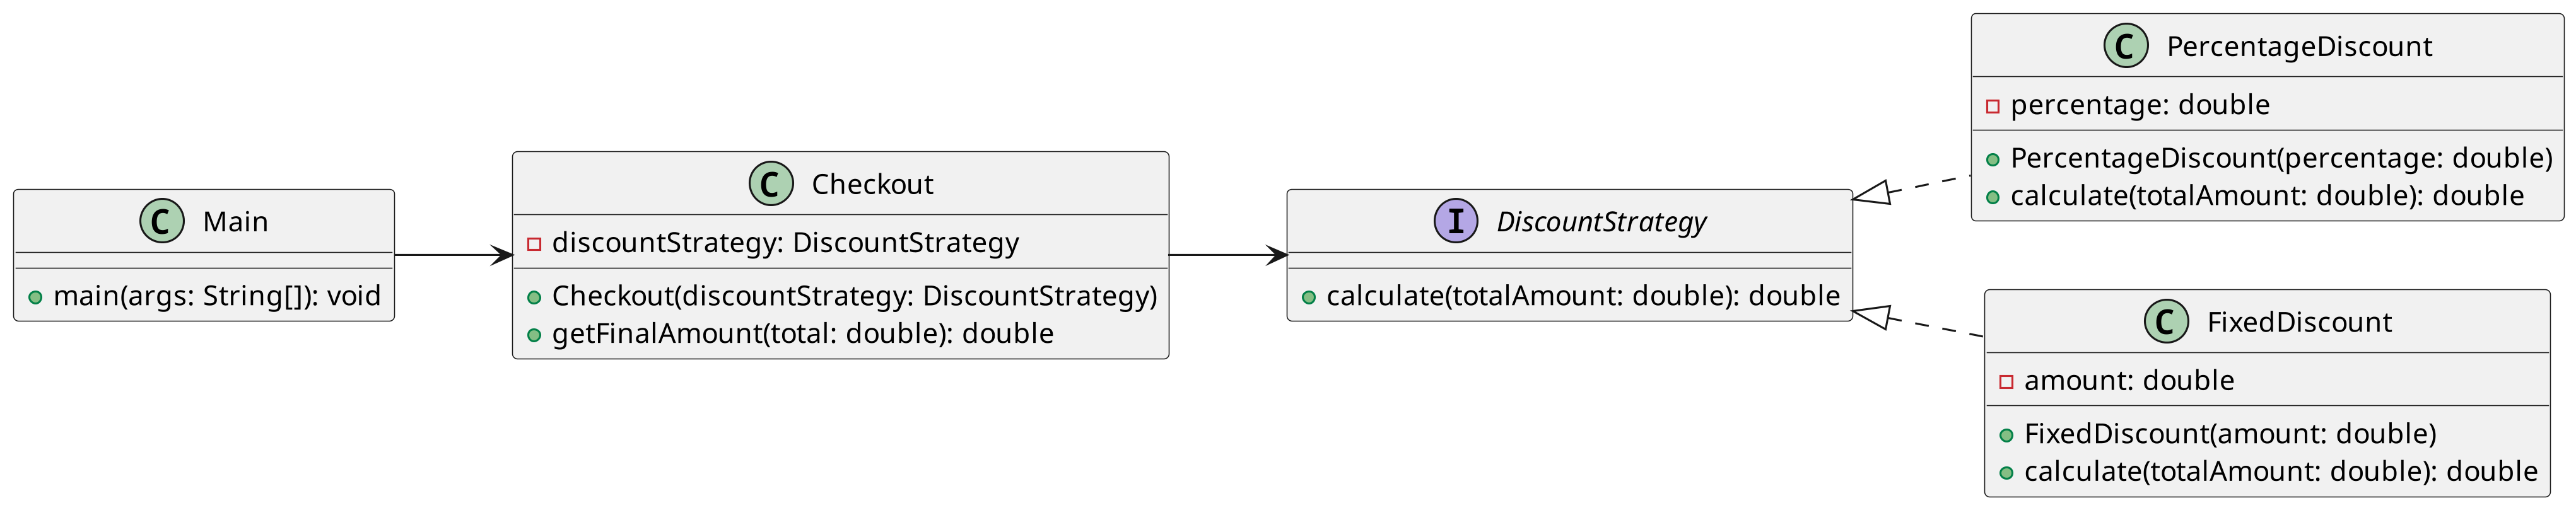
\includegraphics[width=\textwidth]{../../figures/out/strategy.png}
	\vspace{5pt}
	
	\small Gambar menunjukkan bagaimana \texttt{Context} menggunakan \texttt{Strategy} dan berinteraksi dengan implementasi konkret yang dapat diganti-ganti.
\end{frame}

\begin{frame}[fragile]{Strategy: Antarmuka Strategy}
	\vspace{5pt}
	\begin{lstlisting}[style=JavaStyle]
		public interface DiscountStrategy {
			double calculate(double totalAmount);
		}
	\end{lstlisting}
	\vspace{4pt}
	\small Antarmuka \texttt{DiscountStrategy} mendefinisikan kontrak umum bagi semua strategi diskon yang dapat digunakan oleh \texttt{Context}.
\end{frame}

\begin{frame}[fragile]{Strategy: Implementasi Diskon Persentase}
	\vspace{5pt}
	\begin{lstlisting}[style=JavaStyle]
		public class PercentageDiscount implements DiscountStrategy {
			private double percentage;
			
			public PercentageDiscount(double percentage) {
				this.percentage = percentage;
			}
			
			@Override
			public double calculate(double totalAmount) {
				return totalAmount * (1 - percentage);
			}
		}
	\end{lstlisting}
	\vspace{4pt}
	\small Strategi ini menghitung potongan harga berdasarkan persentase dari total belanja.
\end{frame}

\begin{frame}[fragile]{Strategy: Implementasi Diskon Tetap}
	\vspace{5pt}
	\begin{lstlisting}[style=JavaStyle]
		public class FixedDiscount implements DiscountStrategy {
			private double amount;
			
			public FixedDiscount(double amount) {
				this.amount = amount;
			}
			
			@Override
			public double calculate(double totalAmount) {
				return totalAmount - amount;
			}
		}
	\end{lstlisting}
	\vspace{4pt}
	\small Strategi ini mengurangi nilai total dengan angka tetap berapa pun nilai transaksi.
\end{frame}

\begin{frame}[fragile]{Strategy: Context (Kasir)}
	\vspace{5pt}
	\begin{lstlisting}[style=JavaStyle]
		public class Checkout {
			private DiscountStrategy discountStrategy;
			
			public Checkout(DiscountStrategy discountStrategy) {
				this.discountStrategy = discountStrategy;
			}
			
			public double getFinalAmount(double total) {
				return discountStrategy.calculate(total);
			}
		}
	\end{lstlisting}
	\vspace{4pt}
	\small \texttt{Checkout} bertanggung jawab menghitung total harga akhir dengan menggunakan strategi diskon yang dipilih.
\end{frame}

\begin{frame}[fragile]{Strategy: Client (Penggunaan Strategi Diskon)}
	\vspace{10pt}
	\begin{lstlisting}[style=JavaStyle]
		public class Main {
			public static void main(String[] args) {
				double total = 100.0;
				
				// Diskon persentase
				DiscountStrategy percentage = new PercentageDiscount(0.2);
				Checkout checkout1 = new Checkout(percentage);
				System.out.println("Diskon persentase: " +
				checkout1.getFinalAmount(total));
				
				// Diskon tetap
				DiscountStrategy fixed = new FixedDiscount(15.0);
				Checkout checkout2 = new Checkout(fixed);
				System.out.println("Diskon tetap: " +
				checkout2.getFinalAmount(total));
			}
		}
	\end{lstlisting}
	\vspace{4pt}
	\small Klien dapat memilih strategi diskon yang digunakan tanpa mengubah struktur kode utama.
\end{frame}

\section{Pola Command}

\begin{frame}{\hfill}
	\centering
	\textbf{\Huge{Pola Command}}
\end{frame}


\begin{frame}{Command: Tujuan dan Konteks Penggunaan}
	\vspace{15pt}
	Pola \textit{Command} membungkus permintaan sebagai objek yang dapat diantrikan atau dibatalkan, untuk kelola perintah tanpa ubah logika.
	\vspace{1pt}
	\begin{columns}[T]
		\column{0.5\textwidth}
		\textbf{Tujuan:}
		\begin{itemize}
			\item Pisahkan \texttt{Invoker} dan \texttt{Receiver}.
			\item Dukung undo/redo dan pencatatan.
			\item Kelola makro dan antrean tugas.
		\end{itemize}
		
		\textbf{Struktur:}
		\begin{itemize}
			\item \textbf{Command:} Antarmuka perintah.
			\item \textbf{ConcreteCommand:} Isi perintah.
			\item \textbf{Receiver:} Eksekutor aksi.
			\item \textbf{Invoker:} Pemicu.
			\item \textbf{Client:} Pengatur hubungan.
		\end{itemize}
		
		\column{0.5\textwidth}
		\textbf{Kapan Dipakai:}
		\begin{itemize}
			\item Perlu undo, log, atau penjadwalan.
			\item Banyak permintaan dinamis.
			\item Perintah kompleks perlu dikemas.
		\end{itemize}
		
		\textbf{Contoh:}
		\begin{itemize}
			\item GUI: tombol sebagai \texttt{Command}.
			\item Remote untuk perangkat rumah.
			\item Game/editor: undo, redo, makro.
			\item Task queue dan job scheduler.
		\end{itemize}
	\end{columns}
\end{frame}

\begin{frame}{Command: Contoh Kasus Penggunaan}
	\vspace{20pt}
	Pola \textit{Command} membungkus aksi sebagai objek, memisahkan pemicu dan pelaksana, serta memungkinkan undo, redo, antrian, dan pencatatan. Berikut contoh penggunaannya:
	
	\vspace{6pt}
	\begin{itemize}
		\item \textbf{Tombol GUI:} Aksi seperti \texttt{Save} dan \texttt{Undo} direpresentasikan sebagai objek.
		
		\item \textbf{Remote Control:} Tombol dikaitkan ke perintah seperti nyalakan lampu atau AC.
		
		\item \textbf{Game:} Aksi seperti \texttt{Move} dan \texttt{Attack} disimpan sebagai objek untuk replay.
		
		\item \textbf{Undo/Redo:} Perubahan dibatalkan atau diulang dari stack perintah.
		
		\item \textbf{Job Queue:} Tugas dijalankan satu per satu dari antrean perintah.
		
		\item \textbf{Saga Pattern:} Transaksi antar layanan dikemas dalam perintah dan bisa dikompensasi.
		
		\item \textbf{Logging:} Perintah dicatat lengkap untuk audit.
	\end{itemize}
\end{frame}


\begin{frame}{Command: Kelebihan dan Kekurangan}
	\vspace{10pt}
	Pola \textit{Command} membungkus permintaan sebagai objek untuk mendukung undo/redo, logging, makro, dan penjadwalan. Cocok untuk sistem kompleks, tetapi bisa berlebihan untuk tugas sederhana atau sistem kecil.
	
	\vspace{6pt}
	\begin{columns}[T]
		\column{0.5\textwidth}
		\textbf{Kelebihan:}
		\begin{itemize}
			\item Pisahkan \texttt{Invoker} dan \texttt{Receiver}, dukung modularitas.
			\item Undo/redo mudah lewat riwayat perintah.
			\item Strategi baru cukup tambahkan \texttt{ConcreteCommand}.
			\item Mendukung makro dan scripting.
			\item Bisa diantrikan atau dijadwalkan.
		\end{itemize}
		
		\column{0.5\textwidth}
		\textbf{Kekurangan:}
		\begin{itemize}
			\item Banyak kelas jika perintah beragam.
			\item Terlalu kompleks untuk aksi sederhana.
			\item Undo butuh simpan status lama.
			\item Klien perlu pemetaan manual ke perintah.
			\item Debugging/tracing jadi lebih sulit.
		\end{itemize}
	\end{columns}
\end{frame}

\begin{frame}{Struktur Pola Command}
	\vspace{10pt}
	\centering
	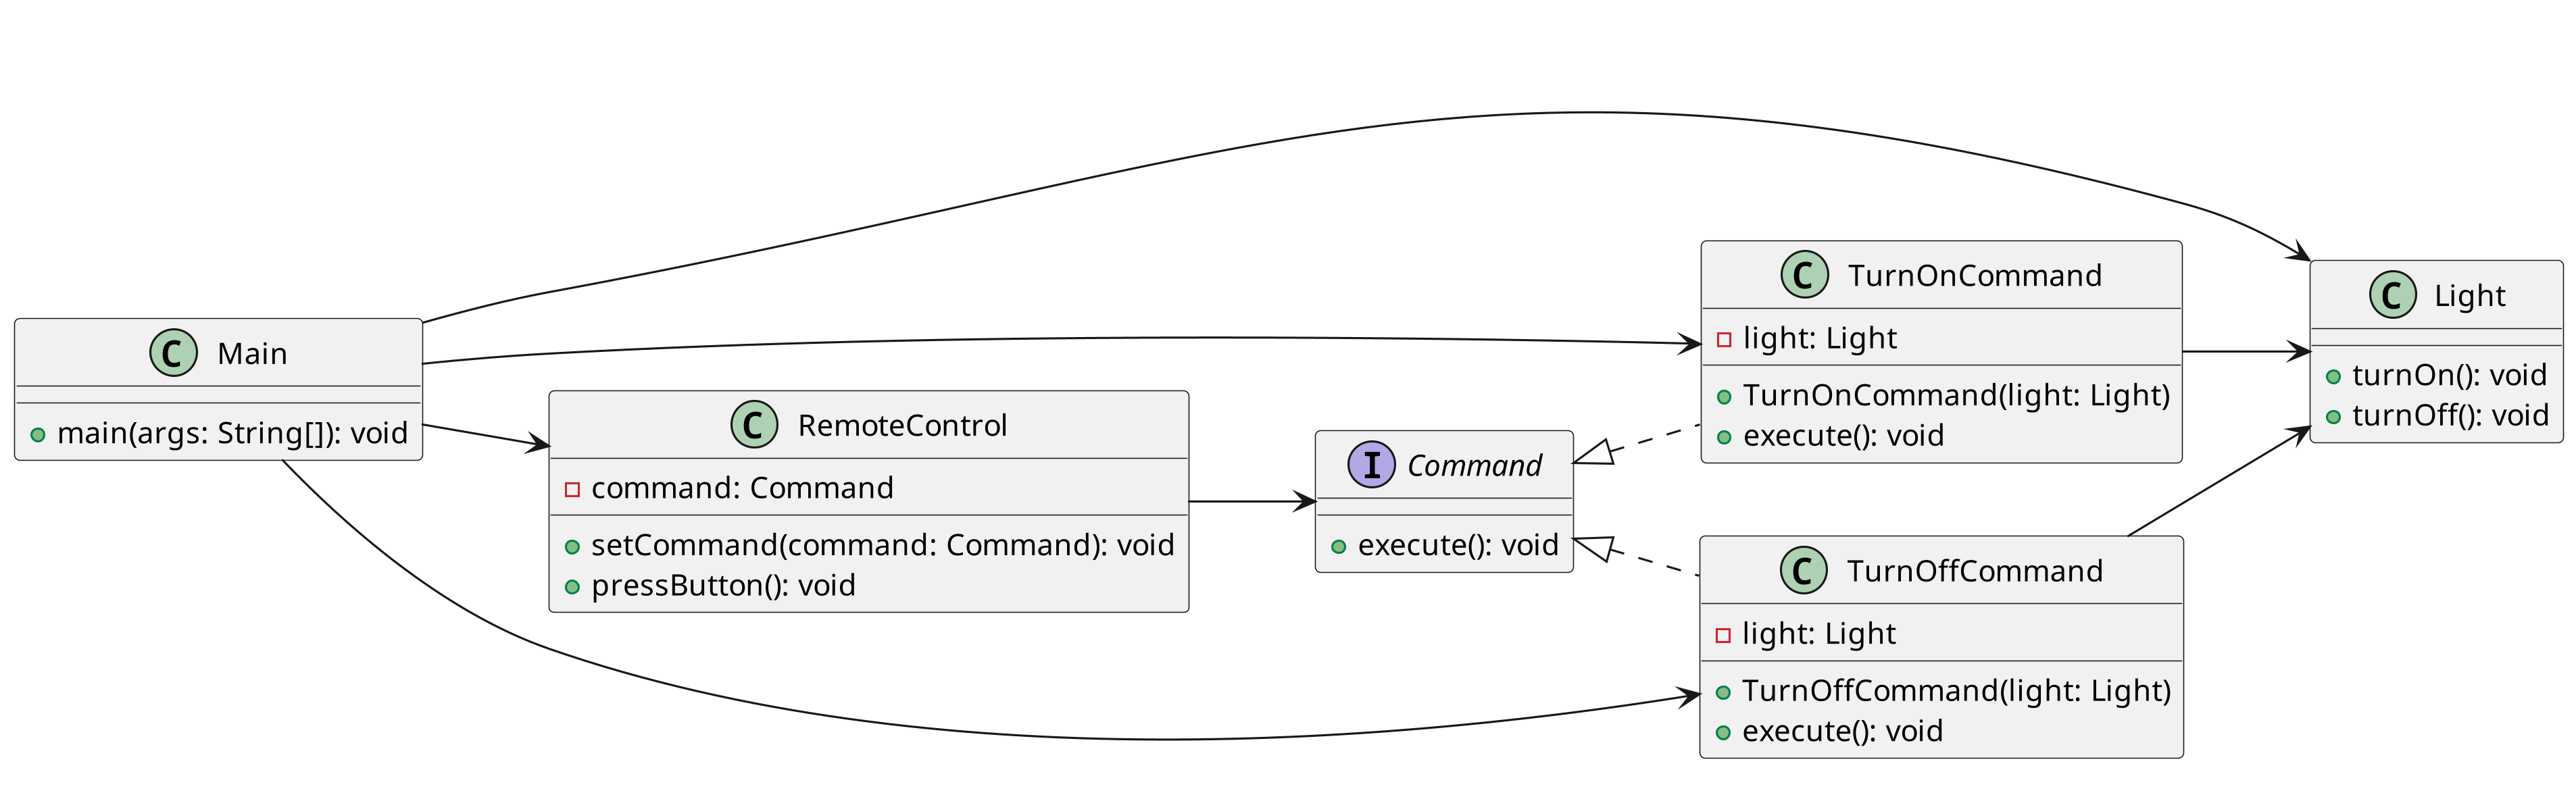
\includegraphics[width=\textwidth]{../../figures/out/command.png}
	
	\vspace{6pt}
	\small Diagram menunjukkan peran \texttt{Client}, \texttt{Invoker}, \texttt{Command}, \texttt{ConcreteCommand}, dan \texttt{Receiver} dalam pola Command.
\end{frame}

\begin{frame}[fragile]{Command: Antarmuka Perintah}
	\begin{lstlisting}[style=JavaStyle]
		public interface Command {
			void execute();
		}
	\end{lstlisting}
	\small Antarmuka \texttt{Command} mendefinisikan kontrak umum untuk semua perintah yang dapat dieksekusi.
\end{frame}

\begin{frame}[fragile]{Receiver: Lampu}
	\begin{lstlisting}[style=JavaStyle]
		public class Light {
			public void turnOn() {
				System.out.println("Lampu dinyalakan.");
			}
			public void turnOff() {
				System.out.println("Lampu dimatikan.");
			}
		}
	\end{lstlisting}
	\small Kelas \texttt{Light} menyimpan logika aksi nyata, yaitu menyalakan dan mematikan lampu.
\end{frame}

\begin{frame}[fragile]{ConcreteCommand: Menyalakan Lampu}
	\begin{lstlisting}[style=JavaStyle]
		public class TurnOnCommand implements Command {
			private Light light;
			public TurnOnCommand(Light light) {
				this.light = light;
			}
			public void execute() {
				light.turnOn();
			}
		}
	\end{lstlisting}
	\small \texttt{TurnOnCommand} menyimpan referensi ke \texttt{Light} dan mengeksekusi metode \texttt{turnOn()}.
\end{frame}

\begin{frame}[fragile]{ConcreteCommand: Mematikan Lampu}
	\begin{lstlisting}[style=JavaStyle]
		public class TurnOffCommand implements Command {
			private Light light;
			public TurnOffCommand(Light light) {
				this.light = light;
			}
			public void execute() {
				light.turnOff();
			}
		}
	\end{lstlisting}
	\small \texttt{TurnOffCommand} memanggil metode \texttt{turnOff()} pada objek lampu yang dikendalikan.
\end{frame}

\begin{frame}[fragile]{Invoker: RemoteControl}
	\begin{lstlisting}[style=JavaStyle]
		public class RemoteControl {
			private Command command;
			public void setCommand(Command command) {
				this.command = command;
			}
			public void pressButton() {
				command.execute();
			}
		}
	\end{lstlisting}
	\small \texttt{RemoteControl} bertindak sebagai pemicu perintah tanpa tahu detail implementasi perintah.
\end{frame}

\begin{frame}[fragile]{Client: Menjalankan Perintah}
	\begin{lstlisting}[style=JavaStyle]
		public class Main {
			public static void main(String[] args) {
				Light lampu = new Light();
				Command on = new TurnOnCommand(lampu);
				Command off = new TurnOffCommand(lampu);
				
				RemoteControl remote = new RemoteControl();
				remote.setCommand(on);
				remote.pressButton(); // Nyalakan
				
				remote.setCommand(off);
				remote.pressButton(); // Matikan
			}
		}
	\end{lstlisting}
	\small \texttt{Main} mengatur hubungan antar objek dan mengeksekusi perintah melalui \texttt{RemoteControl}.
\end{frame}

\begin{frame}{Kesimpulan}
	\vspace{10pt}
	Keempat pola desain perilaku yang dibahas—\textit{Interpreter}, \textit{Observer}, \textit{Strategy}, dan \textit{Command}—memberikan solusi spesifik terhadap kebutuhan sistem yang berbeda.
	
	\vspace{8pt}
	\begin{itemize}
		\item \textbf{Interpreter:} Mengevaluasi ekspresi atau DSL dengan struktur grammar stabil. Cocok untuk kalkulator, query mini, atau aturan logika.
		
		\item \textbf{Observer:} Menyebarkan notifikasi ke banyak objek saat status berubah. Mendukung sistem event-driven dan MVC.
		
		\item \textbf{Strategy:} Memisahkan algoritma dari penggunaannya. Cocok untuk variasi logika runtime seperti diskon, pengurutan, atau kompresi.
		
		\item \textbf{Command:} Membungkus aksi sebagai objek. Mendukung undo/redo, penjadwalan, logging, dan kontrol terpusat.
	\end{itemize}
	
	\vspace{6pt}
	Pemilihan pola yang tepat mendorong arsitektur yang fleksibel, modular, dan mudah dipelihara.
\end{frame}



%\section{Pola Facade}

%\begin{frame}{\hfill}
%	\centering
%	\textbf{\Huge{Pola Facade}}
%\end{frame}


\end{document}
                                                                                                                                                                               